To elucidate the impact of cellular stimulation with activators of the innate immune response and human Respiratory Syncytial Virus (hRSV) on the expression of human Interferon-Induced Protein with Tetratricopeptide Repeats (IFIT) genes, a quantitative real-time reverse transcription polymerase chain reaction (RT-qPCR) analysis was carried out in accordance with the methodology delineated in Section \ref{sec:Quantitative Real Time/Reverse Transcription PCR}. In summary, cells were cultivated in 12-well plates and subsequently exposed to the respective stimulants. At the endpoint of the experiments, RNA extraction was performed, followed by complementary DNA (cDNA) synthesis and transcript quantification through qPCR. All transcript levels were normalized to the expression of human Glyceraldehyde-3-Phosphate Dehydrogenase (GAPDH) gene using the \(\Delta\)\(\Delta\)Ct method. Subsequently, all values were further normalized against mock-treated samples, facilitating data consolidation and inter-experimental induction value comparisons. The statistical analysis adhered to the procedures outlined in Section \ref{sec:Statistical Analysis}. It is important to note that the selection of the appropriate statistical test was contingent upon the assessment of data distribution normality and the equality of variance, considerations that will be elaborated upon in the subsequent sections of this chapter.

\subsection{Human \textit{IFITs} Responses of to Activators of Innate Immune Response} \label{subsec:Human IFIT Responses to Activators of Innate Immune Response}
In order to establish the expression competency of human \textit{IFITs} of the A549 cell line, along with elucidating how different innate immune pathways contribute to the overall expression profile, I treated the cells with differing activators of the innate immune response. As described in Section \ref{subsec:Routes of IFIT Expression Activation}, and depicted in Figure \ref{fig:Pathways Inducing ISG mRNA Production.},  interferon-stimulated genes (ISGs) can have their induction activated either via the interferon receptor signalling, intracellular foreign nucleic acid detection or via extracellular PAMP sensing. The latter, in the context of RSV, includes stimulation of TLR4 with either LPS or RSV particles. After surveying the literature I ended up using 1,000 international units (IU) per mL of human interferon alpha (\cite{Terenzi2006DistinctISG56}; \cite{Santhakumar2018ChickenViruses}). For interferon-gamma stimulation, which stimulates predominantly immune cells \textit{in vivo} concentrations of 500, 1,000 and 2,000 IU/mL were used. LPS was administered in concentrations of 5 ng/mL and 5 \(\mu\)g/mL for the duration of 6 hours. (\cite{Mears2019Ifit1Cells}; \cite{Zhang2019GrouperResponse}). To stimulate intracellular foreign nucleic acid recognition 2 \(\mu\)g of poly I:C were transfected into A549 cells and incubated for 24 hours (\cite{Mears2019Ifit1Cells}; \cite{Palchetti2015TransfectedCells}).

\begin{figure}
    \centering
    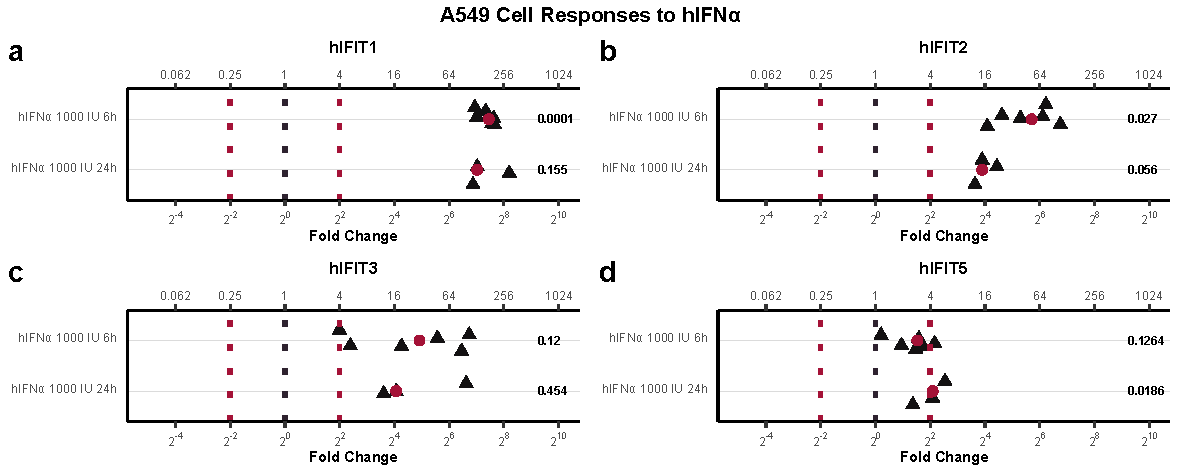
\includegraphics[width=1\linewidth]{06. Chapter 1/Figs/01. Induction/01. a549_treat_ifna.pdf}
    \caption[\textit{hIFIT} Gene Expression in A549 Cells in Response to hIFN\(\alpha\) Stimulation.]{\textbf{\textit{hIFIT} Gene Expression in A549 Cells in Response to hIFN\(\alpha\) Stimulation.} (a) \textit{hIFIT1}, (b) \textit{hIFIT2}, (c) \textit{hIFIT3}, and (d) \textit{hIFIT5} gene expression levels were assessed using quantitative real-time PCR (qPCR) in A549 cells following stimulation with human interferon alpha (hIFN\(\alpha\)) at a concentration of 1000 IU/mL for either 6 or 24 hours. Relative expression values are normalized to standardized mock-treated samples. Median values are represented by red circles. The black dotted line represents mock expression levels, while the red dotted lines indicate biologically significant induction thresholds. Numeric values indicate the p-values compared to mock-treated samples.}
    \label{fig:A549 Response to hIFNa}
\end{figure}

The A549 cell line, originally derived from lung carcinomatous tissue of a 58-year-old Caucasian male in 1972, has established itself as a robust model for alveolar epithelial cells and is routinely employed in both cancer and viral research (\cite{Lieber1976ACells}). In our investigations, upon subjecting the A549 cell line to stimulation with 1,000 IU/mL of hIFN\(\alpha\), administered for either 6 or 24 hours, notable alterations in the expression of human \textit{IFIT1}, \textit{IFIT2}, and \textit{IFIT3} were observed, particularly in the case of \textit{hIFIT1}. The induction of \textit{hIFIT1} surpassed 200-fold (as depicted in Figure \ref{fig:A549 Response to hIFNa}). The relative induction levels were fairly consistent between \textit{hIFIT2} and \textit{hIFIT3} at 50-fold and 32-fold at 6 hours for \textit{hIFIT2} and \textit{hIFIT3} respectively, and 16-fold at 24 hours. For all three of these \textit{hIFIT} genes, an intriguing trend emerged, where prolonged incubation with hIFN\(\alpha\) led to a decline in expression, approximately halving the induction levels compared to the 6-hour incubation period. In contrast, human \textit{IFIT5} exhibited minimal induction compared to the other \textit{hIFIT} members, with induction levels reaching 3-fold and 4-fold for the 6-hour and 24-hour incubation periods, respectively. This level of induction approaches the threshold considered biologically significant, particularly for Interferon-Stimulated Genes (ISGs), which are generally characterized by low basal expression levels. Additionally, a distinct temporal pattern was evident in hIFIT5 induction, showcasing a reversed dependency on incubation time with hIFN\(\alpha\). These findings collectively suggest varying degrees of induction sensitivity among the IFIT family members, with \textit{hIFIT1} displaying high sensitivity to induction, \textit{hIFIT2} and \textit{hIFIT3} demonstrating intermediate induction levels, and \textit{hIFIT5} exhibiting lower induction levels. Importantly, it is noteworthy that all \textit{hIFIT} gene expression values conformed to normal distributions with unequal variances, with the exception of \textit{hIFIT5}, which displayed normal distribution but exhibited equal variance. 

\begin{figure}
    \centering
    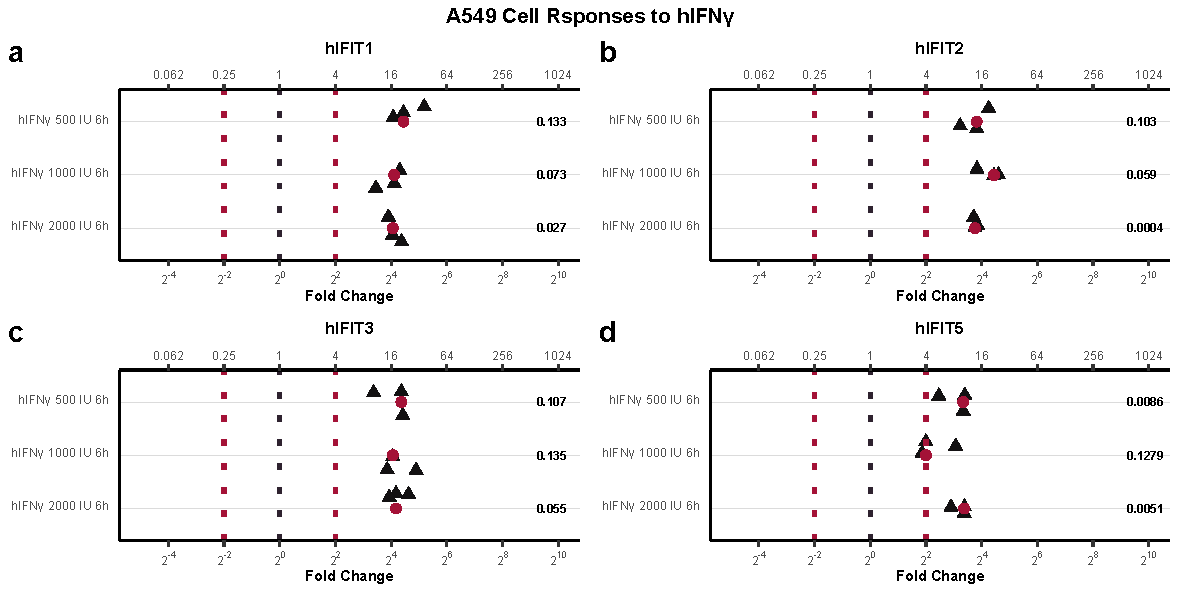
\includegraphics[width=1\linewidth]{06. Chapter 1/Figs/01. Induction/02. a549_treat_ifng.pdf}
    \caption[\textit{hIFIT} Gene Expression in A549 Cells in Response to hIFN\(\gamma\) Stimulation.]{\textbf{\textit{hIFIT} Gene Expression in A549 Cells in Response to hIFN\(\gamma\) Stimulation.} (a) \textit{hIFIT1}, (b) \textit{hIFIT2}, (c) \textit{hIFIT3}, and (d) \textit{hIFIT5} gene expression levels were assessed using quantitative real-time PCR (qPCR) in A549 cells following stimulation with human interferon gamma (hIFN\(\gamma\)) at concentrations of 500, 1000, and 2000 IU/mL for 6 hours. Relative expression values are normalized to standardized mock-treated samples. Median values are represented by red circles. The black dotted line represents mock expression levels, while the red dotted lines indicate biologically significant induction thresholds. Numeric values indicate the p-values compared to mock-treated samples.}
    \label{fig:A549 Response to hIFNg}
\end{figure}

The response of human \textit{IFIT} genes to human Interferon Gamma (hIFN\(\gamma\)) is presented in Figure \ref{fig:A549 Response to hIFNg}. Notably, all \textit{hIFIT} genes, except for \textit{hIFIT5}, exhibited consistent responses across varying concentrations of hIFN\(\gamma\) (500, 1,000, and 2,000 IU/mL), indicating a concentration-independent induction of approximately 15-fold. In contrast, \textit{hIFIT5} displayed a unique response pattern, demonstrating a 10-fold increase at very low and very high concentrations, with only a 4-fold increase in transcript abundance observed at the 1,000 IU/mL concentration. This observation suggests a relatively uniform interferon-gamma-mediated induction for all \textit{IFIT} genes. Furthermore, the collective data, when considered alongside the findings from hIFN\(\alpha\) induction, affirms the induction capability of the A549 cell line for \textit{hIFIT} genes. This represents a significant aspect of our study. It's important to note that, except for \textit{hIFIT5}, all \textit{hIFIT} gene expression values exhibited normal distributions but with unequal variances. Conversely, \textit{hIFIT5} exhibited both normal distribution and normal variance, highlighting its distinct behavior in this context.

\begin{figure}
    \centering
    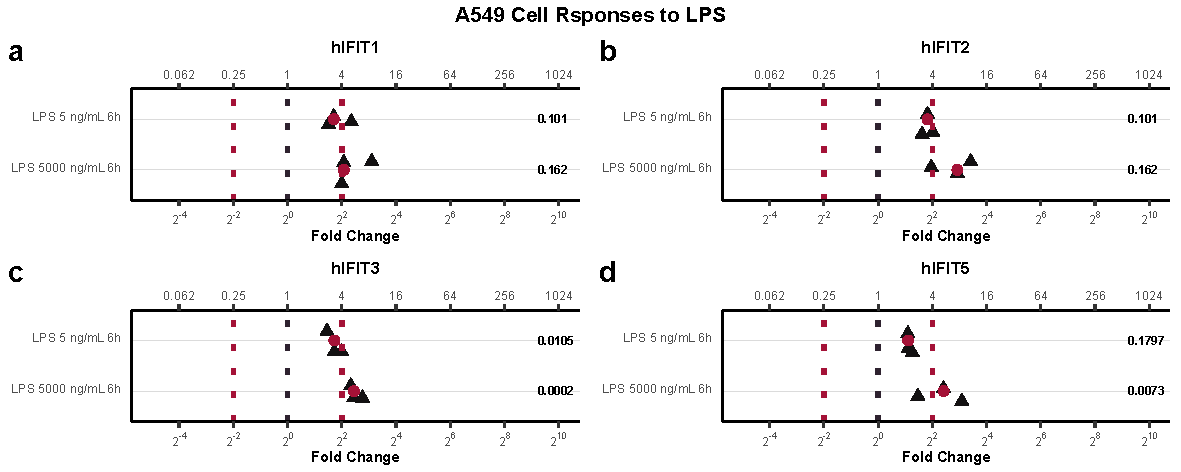
\includegraphics[width=1\linewidth]{06. Chapter 1/Figs/01. Induction/03. a549_treat_lps.pdf}
    \caption[\textit{hIFIT} Gene Expression in A549 Cells in Response to LPS.]{\textbf{\textit{hIFIT} Gene Expression in A549 Cells in Response to LPS.} (a) \textit{hIFIT1}, (b) \textit{hIFIT2}, (c) \textit{hIFIT3}, and (d) \textit{hIFIT5} gene expression levels were assessed using quantitative real-time PCR (qPCR) in A549 cells following stimulation with bacterial lipopolysaccharide (LPS) at concentrations of 5 and 5000 ng/mL for 6 hours. Relative expression values are normalized to standardized mock-treated samples. Median values are represented by red circles. The black dotted line represents mock expression levels, while the red dotted lines indicate biologically significant induction thresholds. Numeric values indicate the p-values compared to mock-treated samples.}
    \label{fig:A549 Response to LPS}
\end{figure}

To investigate the involvement of Toll-like Receptor 4 (TLR4), a receptor known for its role in detecting Respiratory Syncytial Virus (RSV) particles (\cite{Funchal2015RespiratoryNeutrophils}), A549 cells were subjected to a 6-hour incubation period with both low (5 ng/mL) and high (5,000 ng/mL) concentrations of bacterial Lipopolysaccharide (LPS), a known activator of TLR4. Our observations reveal that all \textit{IFITs} exhibit responses in a concentration-dependent manner when exposed to LPS stimulation. However, it's important to note that the magnitude of their response to LPS is comparatively lower than that induced by other stimuli utilized in this study. Specifically, low-concentration LPS incubation led to biologically insignificant induction levels, with a 2-fold increase observed for \textit{hIFIT5} and a 3-fold increase for the other \textit{IFITs}. In contrast, high-concentration LPS stimulation yielded biologically significant induction levels, ranging from 4 to 8-fold induction for the various \textit{hIFITs}. Remarkably, when considering the statistical characteristics, it's noteworthy that, with the exception of \textit{hIFIT3}, all \textit{hIFIT} gene expression values exhibited normal distributions but with unequal variances. Conversely, \textit{hIFIT3} displayed both a normal distribution and normal variance. These findings underscore the nuanced nature of \textit{IFIT} gene responses to TLR4 activation by LPS, shedding light on the intricacies of this signaling pathway within the A549 cell line.

\begin{figure}
    \centering
    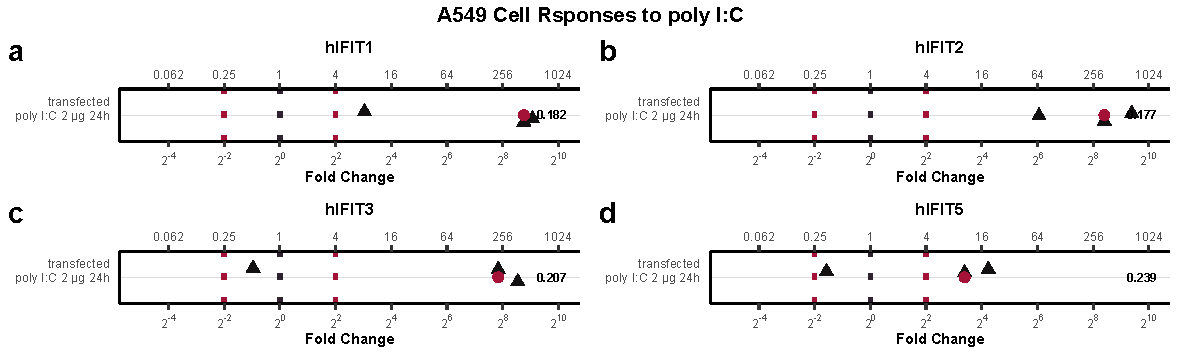
\includegraphics[width=1\linewidth]{06. Chapter 1/Figs/01. Induction/04. a549_treat_polyic.pdf}
    \caption[\textit{hIFIT} Gene Expression in A549 Cells in Response to Transfected poly I:C.]{\textbf{\textit{hIFIT} Gene Expression in A549 Cells in Response to Transfected poly I:C.} (a) \textit{hIFIT1}, (b) \textit{hIFIT2}, (c) \textit{hIFIT3}, and (d) \textit{hIFIT5} gene expression levels were assessed using quantitative real-time PCR (qPCR) in A549 cells following transfection with 2 \(\mu\)g of poly I:C for 24 hours.  Relative expression values are normalized to standardized mock-treated samples. Median values are represented by red circles. The black dotted line represents mock expression levels, while the red dotted lines indicate biologically significant induction thresholds. Numeric values indicate the p-values compared to mock-treated samples.}
    \label{fig:A549 Response to poly I:C}
\end{figure}

Upon transfecting A549 cells with 2 µg of poly I:C for a 24-hour duration, we observed the most significant induction compared to the other inducers employed in our study, as depicted in Figure \ref{fig:A549 Response to poly I:C}. Consistent with the trends observed with other inducers, the induction of \textit{hIFIT1} was the most pronounced, reaching approximately 500-fold, followed by \textit{hIFIT2} and \textit{hIFIT3} with respective induction levels of approximately 300-fold and 200-fold. In contrast, \textit{hIFIT5} exhibited the lowest response, with an induction of only 10-fold. These findings reinforce the notion that \textit{hIFIT5} appears to be subject to distinct transcriptomic regulation compared to the other members of the \textit{IFIT} gene family. Importantly, it's worth noting that all \textit{hIFIT} gene expression values exhibited normal distributions, albeit with unequal variances. 

\begin{figure}
    \centering
    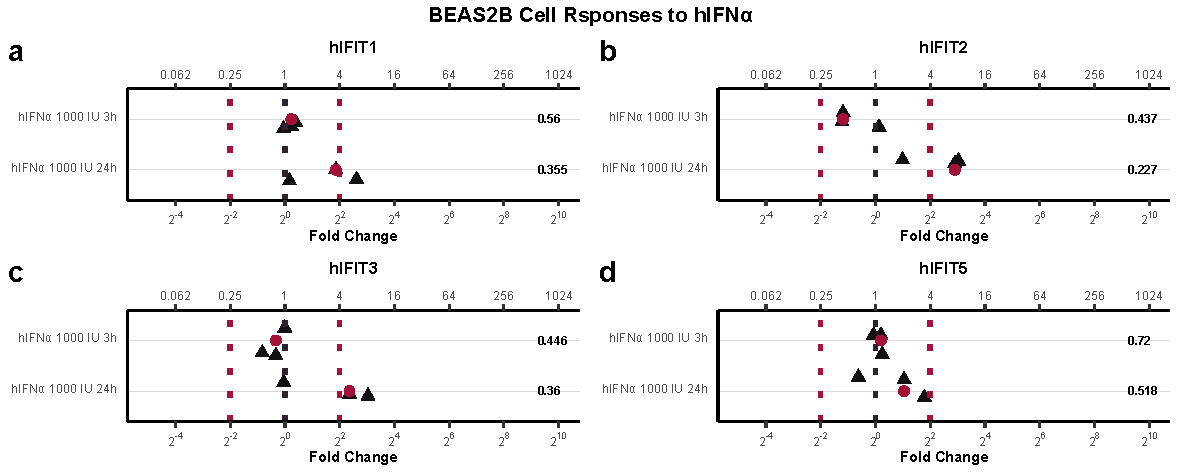
\includegraphics[width=1\linewidth]{06. Chapter 1/Figs/01. Induction/09. beas2b_ifna.pdf}
    \caption[\textit{hIFIT} Gene Expression in BEAS-2B Cells in Response to hIFN\(\alpha\) Stimulation.]{\textbf{\textit{hIFIT} Gene Expression in BEAS-2B Cells in Response to hIFN\(\alpha\) Stimulation.} a) \textit{hIFIT1}, (b) \textit{hIFIT2}, (c) \textit{hIFIT3}, and (d) \textit{hIFIT5} gene expression levels were assessed using quantitative real-time PCR (qPCR) in BEAS-2B cells following stimulation with human interferon alpha (hIFN\(\alpha\)) at a concentration of 1000 IU/mL for either 3 or 24 hours. Relative expression values are normalized to standardized mock-treated samples. Median values are represented by red circles. The black dotted line represents mock expression levels, while the red dotted lines indicate biologically significant induction thresholds. Numeric values indicate the p-values compared to mock-treated samples.}
    \label{fig:BEAS-2B responses to hIFNa}
\end{figure}

In an effort to validate the induction data for human interferon alpha (hIFN\(\alpha\)) in a context more biologically relevant model, we turned to the BEAS-2B cell line. Originating from bronchial epithelial biopsies sourced from healthy samples, these cells were later immortalized through the transfection of cyclin-dependent kinase 4 and human telomerase reverse transcriptase, rendering them a valuable resource in the field of bronchial development and pathogenesis (\cite{Ramirez2004ImmortalizationOncoproteins}). Upon treating BEAS-2B cells with hIFN\(\alpha\) at concentrations of 1,000 IU/mL for a brief 3-hour duration, our observations indicated that this stimulation was insufficient to induce the expression of any human \textit{IFIT} genes (as illustrated in Figure \ref{fig:BEAS-2B responses to hIFNa}). However, extending the stimulation period to 24 hours revealed noteworthy induction levels above the threshold of biological significance for \textit{hIFIT1}, \textit{hIFIT2}, and \textit{hIFIT3}, with respective increases of 4-fold, 8-fold, and 5-fold. In contrast, \textit{hIFIT5} exhibited a median induction of only 2-fold. Similar to our observations with the A549 cell line, the behavior of \textit{hIFIT5} in BEAS-2B cells diverged from that of the other human \textit{IFIT} genes. All \textit{hIFIT} values had normal distributions and unequal variance.

\subsection{Human \textit{IFITs} Responses to Human RSV Infection} \label{subsec:Human IFITs Responses to Human RSV}
Having successfully established the \textit{hIFIT} induction competence in our A549 and BEAS-2B cell lines, our attention now shifts towards exploring the impact of human Respiratory Syncytial Virus (hRSV) infection on \textit{hIFIT} induction—a topic that, to date, has remained uninvestigated. To characterize this effect comprehensively, we initially aimed to assess the influence of varying infection multiplicities and durations on \textit{hIFIT} induction, specifically utilizing low, medium, and high multiplicities of infection (MOI) of 0.1, 1, and 2, as well as short and long-term infection durations of 24 and 48 hours post-infection (HPI), respectively. This choice of infection parameters is based on the established practices of our colleagues in the Viral Glycoproteins Group at the Pirbright Institute, who routinely perform hRSV infections in both A549 and BEAS-2B cell lines (CITATION NEEDED). The virus used in these experiments was prepared and quantified as outlined in Section \ref{subsec:Virus Propagation and Production} and Section \ref{subsec:Virus Quantification by TCID50 Assay}. In brief, infected cells were subjected to sonication, leading to the separation of cell debris through centrifugation, followed by the collection of virus-containing supernatant for titration. Subsequently, A549 cells were exposed to hRSV-containing supernatant at the designated MOIs of 0.1, 1, and 2. Total mRNA was extracted from the samples either 24 or 48 hours post-infection (HPI) and subsequently converted into complementary DNA, following the procedures detailed in Section \ref{subsec:RNA Extraction and cDNA Synthesis}. The quantification of this cDNA was carried out via qPCR, as described in Section \ref{subsec:Quantitative PCR}, and the resulting data were analyzed according to the methods outlined in Section \ref{subsec:Data Processing}. The responses of \textit{hIFITs} in relation to HPI and MOI are presented in Figure \ref{fig:A549 response to hRSV timepoints}. Additionally, a plot quantifying human \textit{RSV N} mRNA serves as a control for viral replication. It's important to note that the relative quantification values of \textit{RSV N} should be interpreted with caution, as they are normalised to mock-infected samples, which are expected to contain no \textit{RSV N} mRNA. Consequently, the actual relative values are influenced by the Ct values detected in the mock samples and should be interpreted accordingly.

\begin{figure}
    \centering
    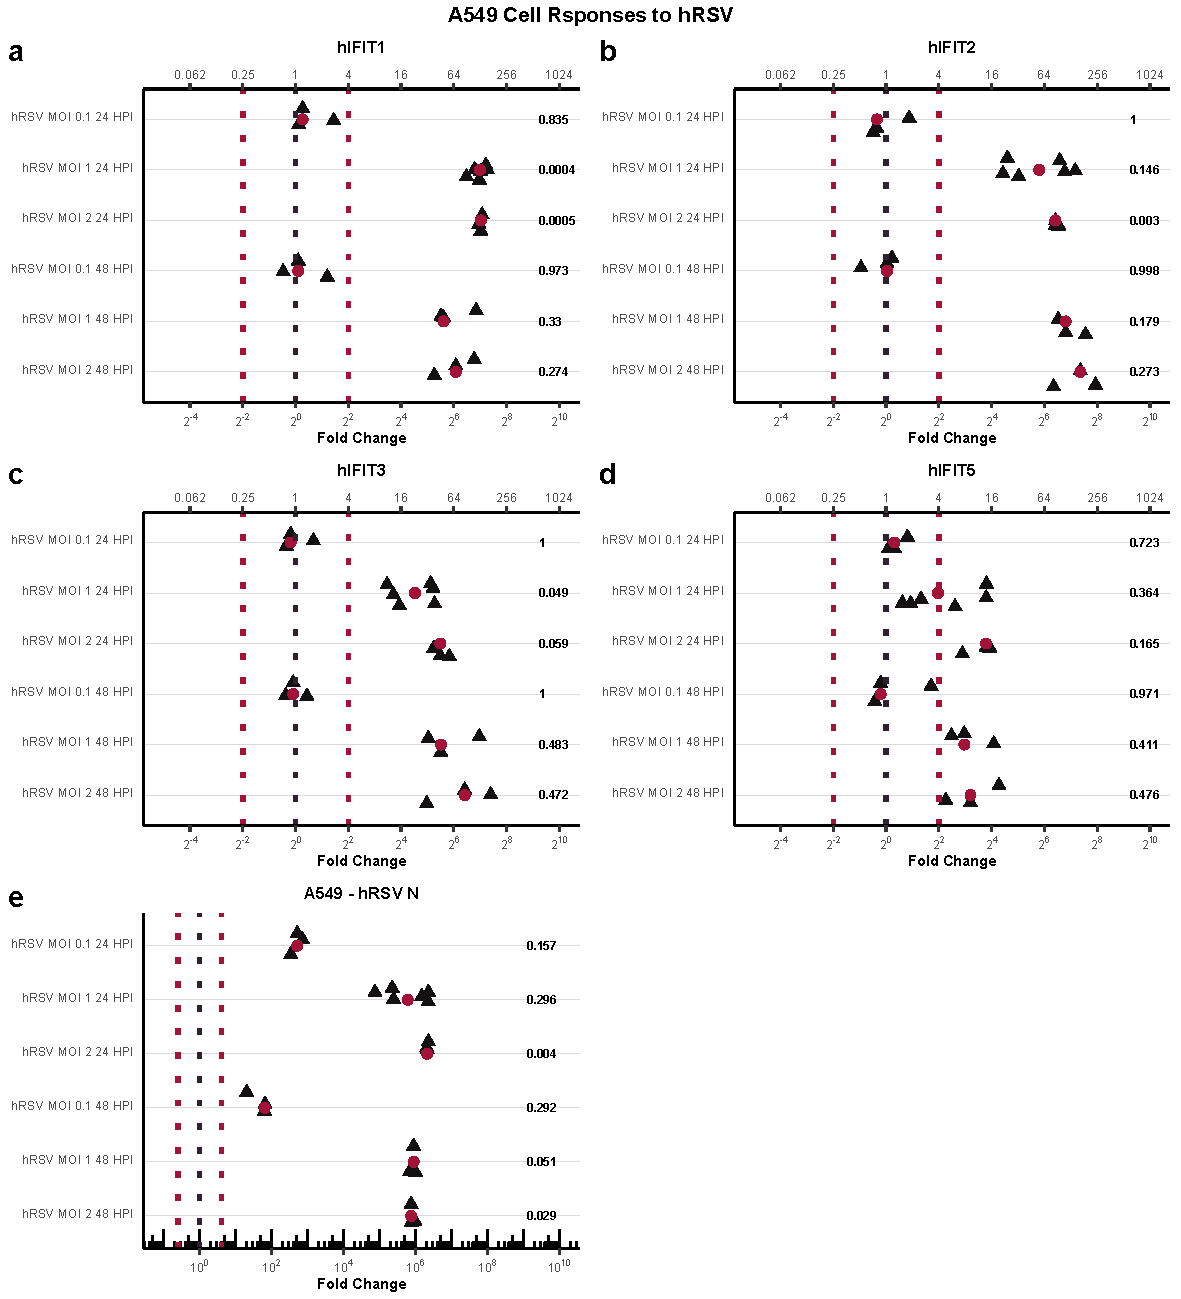
\includegraphics[width=1\linewidth]{06. Chapter 1/Figs/01. Induction/05. a549_hrsv_timepoints.pdf}
    \caption[A549 \textit{hIFIT} Response to hRSV Infection as a Function of Time and MOI.]{\textbf{A549 \textit{hIFIT} Response to hRSV Infection as a Function of Time and MOI.} a) \textit{hIFIT1}, (b) \textit{hIFIT2}, (c) \textit{hIFIT3}, (d) \textit{hIFIT5}, and (e) \textit{hRSV N} gene expression levels were assessed using quantitative real-time PCR (qPCR) in A549 cell line following infection with human RSV at MOI of either 0.1, 1, or 2 for either 24 or 48 hours post-infection. Relative expression values are normalized to standardized mock-treated samples. Median values are represented by red circles. The black dotted line represents mock expression levels, while the red dotted lines indicate biologically significant induction thresholds. Numeric values indicate the p-values compared to mock-treated samples.}
    \label{fig:A549 response to hRSV timepoints}
\end{figure}

Notably, our analysis reveals that low Multiplicity of Infection (MOI) infections, while leading to productive infections as evidenced by relative quantification of \textit{hRSV N} mRNA, did not result in any significant changes in the relative expression levels of \textit{hIFITs}. This observation suggests that the induction of \textit{hIFIT} genes is not solely dependent on viral replication but is influenced by the magnitude of infection. Overall, MOI 2 infections consistently yielded higher induction levels for all \textit{hIFITs} compared to MOI 1 infections. However, the magnitude of induction appeared comparable between the two MOIs. Specifically, \textit{hIFIT1} exhibited the highest induction among the \textit{hIFIT} genes at 24 HPI, with both MOI 1 and 2 infections reaching approximately 120-fold induction levels. At 48 HPI, the induction magnitude slightly decreased, with MOI 1 and 2 infections resulting in median induction values of 50-fold and 80-fold, respectively. This observation underscores the distinct induction dynamics of \textit{hIFIT1} compared to \textit{hIFIT2} and \textit{hIFIT3}. As previously observed in Section \ref{subsec:Human IFIT Responses to Known Activators of Innate Immune Response}, \textit{hIFIT2} and \textit{hIFIT3} displayed similar trends of induction, with \textit{hIFIT2} consistently exhibiting induction levels approximately twice as high as those of \textit{hIFIT3}. Specifically, at 24 HPI, \textit{hIFIT2} displayed inductions of 60-fold and 90-fold for MOIs 1 and 2, respectively, while at 48 HPI, the median induction levels increased to 100-fold and 120-fold, respectively, making \textit{hIFIT2} the highest induced \textit{hIFIT} gene at 48 HPI. Conversely, \textit{hIFIT5} exhibited the lowest induction levels among the \textit{hIFIT} genes, although these inductions were still biologically significant. At 24 HPI, median induction levels for MOIs 1 and 2 were 4-fold and 12-fold, respectively. At 48 HPI, median induction levels for MOIs 1 and 2 were 9-fold and 10-fold, respectively. Importantly, all datasets displayed normal distribution characteristics, albeit with non-equal variances.

\begin{figure}
    \centering
    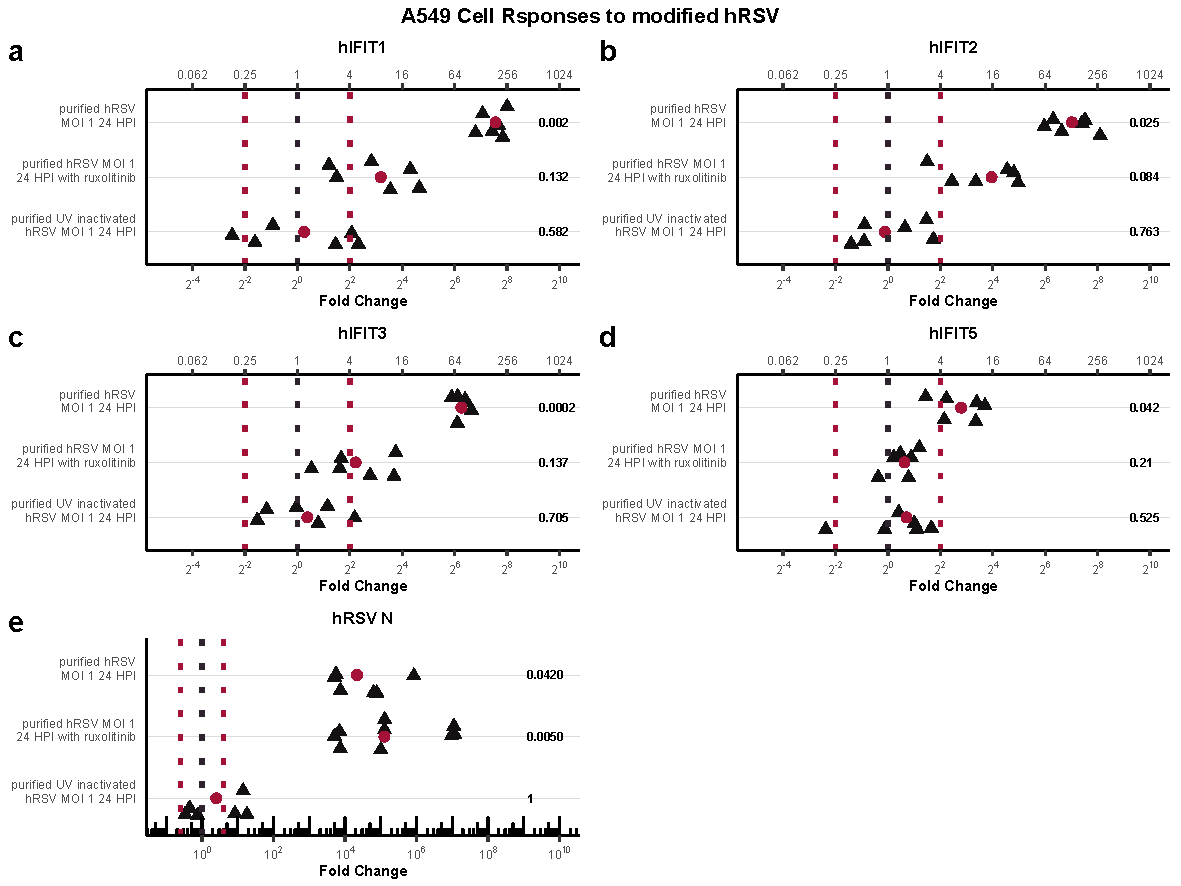
\includegraphics[width=1\linewidth]{06. Chapter 1/Figs/01. Induction/06. a549_hrsv_uv_roxo.pdf}
    \caption[Impact of Ultra-Purification, UV-Inactivation, and INFR Inhibition on \textit{hIFIT} Induction in A549 Cells Following hRSV Infection.]{\textbf{Impact of Ultra-Purification, UV-Inactivation, and INFR Inhibition on \textit{hIFIT} Induction in A549 Cells Following hRSV Infection.}  a) \textit{hIFIT1}, (b) \textit{hIFIT2}, (c) \textit{hIFIT3}, (d) \textit{hIFIT5}, and (e) \textit{hRSV N} gene expression levels were assessed using quantitative real-time PCR (qPCR) in A549 cell line following infection with ultra-purified hRSV at MOI 1 for 24 hours. The cells were subjected to three different conditions: virus infection alone (top row), virus infection in the presence of 5 nM of ruxolitinib (interferon receptor inhibitor) throughout the infection (middle row), or UV-inactivated hRSV infection (bottom row). Relative expression values are normalized to standardized mock-treated samples. Median values are represented by red circles. The black dotted line represents mock expression levels, while the red dotted lines indicate biologically significant induction thresholds. Numeric values indicate the p-values compared to mock-treated samples.}
    \label{fig:The effect of ultra-purification, UV-inactivation and INFR inhibition on hIFIT induction following hRSV infection in A549}
\end{figure}

Following our confirmation of \textit{hIFIT} mRNA expression induced by human Respiratory Syncytial Virus (hRSV) infection, we embarked on an investigation to discern the underlying induction mechanisms. Our primary objective was to ascertain whether the observed induction was a result of hRSV detection or possibly influenced by contaminants present in the virus preparation, such as cytokines, chemokines, or other stimulants. To address this, we produced ultra-purified hRSV preparations through a process involving ultra-centrifugation on a discontinuous sucrose cushion, as meticulously detailed in Section \ref{subsec:Virus Propagation and Production}. Simultaneously, we aimed to shed light on whether the enhanced \textit{hIFIT} expression predominantly occurred within the infected cells as a defense mechanism against acute infection or if the infected cells stimulated neighboring cells to induce \textit{hIFIT} expression as a prophylactic measure. To explore this aspect, we introduced an additional layer of complexity by incubating the cells with 5 nM of ruxolitinib, a well-established small molecule inhibitor of the JAK/STAT pathway, as described in Section \ref{subsec:Viral Infections, UV-Inactivation and Ruxolitinib Treatment}. Furthermore, we also hypothesized that viral replication might be a prerequisite for \textit{hIFIT} expression. To test this hypothesis, we subjected some of the ultra-purified hRSV samples to UV-inactivation using a UV-cross-linker, as described in Section \ref{subsec:Viral Infections, UV-Inactivation and Ruxolitinib Treatment}. Based on our findings from Figure \ref{fig:A549 response to hRSV timepoints}, we elected to employ an MOI of 1 and a 24-hour post-infection (HPI) time point for this experiment, aiming to ensure sufficient \textit{hIFIT} induction while mitigating cellular stress.


The outcomes of this multifaceted experiment are presented in Figure \ref{fig:The effect of ultra-purification, UV-inactivation and INFR inhibition on hIFIT induction following hRSV infection in A549}. Notably, the dataset for \textit{hRSV N} displayed a normal distribution with equal variance, while all other datasets exhibited normal distribution characteristics with non-equal variances. Our findings revealed that ultra-purified hRSV infection, despite yielding lower \textit{hRSV N} mRNA induction levels compared to crude-extracted virus (\(10^6\)-fold to \(10^{4.5}\)-fold; compared to results from Figure \ref{fig:A549 response to hRSV timepoints}), induced the expression of all \textit{hIFITs}, and in some cases, to higher magnitudes than observed with the crude-extracted virus. Specifically, \textit{hIFIT1} and \textit{hIFIT2} exhibited the highest inductions at 180-fold each, compared to 120-fold and 80-fold previously observed, respectively. \textit{hIFIT3} displayed an induction of 75-fold, double the magnitude seen with crude-extracted hRSV, while \textit{hIFIT5} showed a median induction of 6-fold, comparable to the 4-fold induction observed previously. These results strongly suggest that the primary driving force behind \textit{hIFIT} induction is the presence of hRSV and not contaminants within the viral preparation. Regarding the impact of the JAK/STAT inhibitor ruxolitinib, its presence notably reduced the induction of all \textit{hIFITs}. While \textit{hIFIT1}, \textit{hIFIT2}, and \textit{hIFIT3} maintained median induction values above the biologically significant threshold at 8, 10, and 5-fold, respectively, \textit{hIFIT5} exhibited only minimal median induction, approximately 1.5-fold. Additionally, we observed an order of magnitude increase in \textit{hRSV N} mRNA detection, suggesting that inhibiting interferon signaling is advantageous for the virus. Lastly, our investigation into the contribution of non-replicative hRSV particles to \textit{hIFIT} induction revealed that UV-cross-linking of hRSV effectively prevented viral replication, as evidenced by \textit{hRSV N} mRNA quantification. This prevention, in turn, halted the induction of all \textit{hIFITs}, indicating that the recognition of replicative-competent hRSV particles is essential to initiate the signaling cascades leading to \textit{hIFIT} induction. In summary, our findings underscore that hRSV particles play a pivotal role in driving \textit{hIFIT} induction, with viral replication being a crucial factor. Additionally, functional interferon signaling pathways and paracrine interferon signaling initiated by infected cells contribute significantly to the induction process, safeguarding neighboring cells against infection.

\begin{figure}
    \centering
    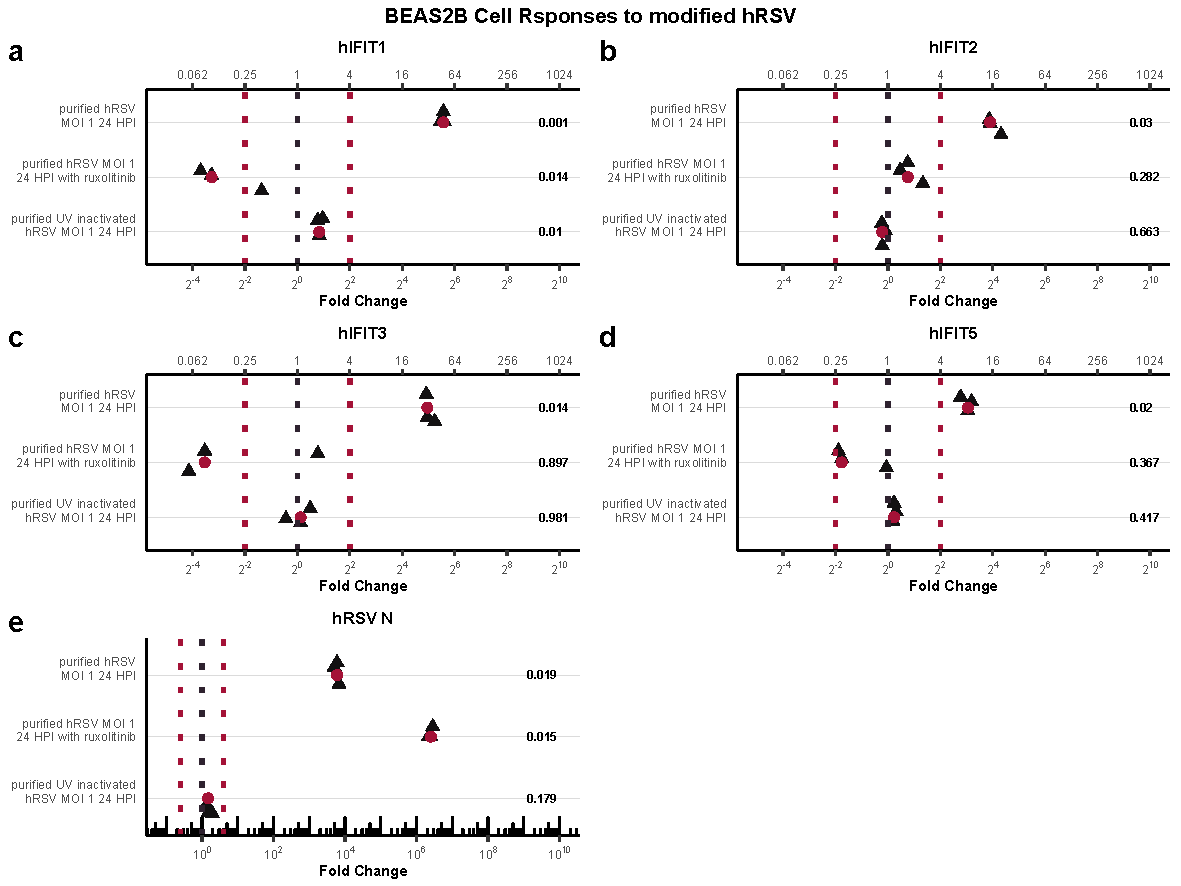
\includegraphics[width=1\linewidth]{06. Chapter 1/Figs/01. Induction/10. beas2b_hrsv.pdf}
    \caption[Impact of Ultra-Purification, UV-Inactivation, and INFR Inhibition on \textit{hIFIT} Induction in BEAS-2B Cells Following hRSV Infection.]{\textbf{Impact of Ultra-Purification, UV-Inactivation, and INFR Inhibition on \textit{hIFIT} Induction in BEAS-2B Cells Following hRSV Infection.}  a) \textit{hIFIT1}, (b) \textit{hIFIT2}, (c) \textit{hIFIT3}, (d) \textit{hIFIT5}, and (e) \textit{hRSV N} gene expression levels were assessed using quantitative real-time PCR (qPCR) in BEAS-2B cell line following infection with ultra-purified hRSV at MOI 1 for 24 hours. The cells were subjected to three different conditions: virus infection alone (top row), virus infection in the presence of 5 nM of ruxolitinib (interferon receptor inhibitor) throughout the infection (middle row), or UV-inactivated hRSV infection (bottom row). Relative expression values are normalized to standardized mock-treated samples. Median values are represented by red circles. The black dotted line represents mock expression levels, while the red dotted lines indicate biologically significant induction thresholds. Numeric values indicate the p-values compared to mock-treated samples.}
    \label{fig:The effect of ultra-purification, UV-inactivation and INFR inhibition on hIFIT induction following hRSV infection in BEAS-2B}
\end{figure}

To further substantiate our findings, we sought validation in the BEAS-2B cell line. We replicated the experiment conducted in Figure \ref{fig:The effect of ultra-purification, UV-inactivation and INFR inhibition on hIFIT induction following hRSV infection in A549}, and the results are documented in Figure \ref{fig:The effect of ultra-purification, UV-inactivation and INFR inhibition on hIFIT induction following hRSV infection in BEAS-2B}. Notably, all datasets in this analysis exhibited normal distribution characteristics with non-equal variances. Our observations revealed that all \textit{hIFITs} were induced to biologically significant levels following infection with ultra-purified hRSV, with inductions of 40-fold, 15-fold, 32-fold, and 7-fold for \textit{hIFIT1}, \textit{hIFIT2}, \textit{hIFIT3}, and \textit{hIFIT5}, respectively. These induction levels markedly exceeded those observed with human interferon alpha treatment, as illustrated in Figure \ref{fig:BEAS-2B responses to hIFNa}. Consistent with our findings in the A549 cell line, \textit{hIFIT1} exhibited the highest induction, while \textit{hIFIT5} demonstrated the weakest response to infection. Intriguingly, \textit{hIFIT3} displayed a higher median induction compared to \textit{hIFIT2} in this context. Upon scrutinizing the impact of ruxolitinib, we noted that it not only prevented the induction of \textit{hIFIT2} but also significantly diminished the relative expression levels of \textit{hIFIT1}, \textit{hIFIT3}, and \textit{hIFIT5} to approximately \(2^{-3}\), \(2^{-3.5}\), and \(2^{-2}\), respectively. This finding suggests that interferon signaling is not only required for \textit{hIFIT2} induction but is also vital for maintaining basal \textit{hIFIT1}, \textit{hIFIT3}, and \textit{hIFIT5} expression levels in the BEAS-2B cell line. Finally, when BEAS-2B cells were exposed to UV-irradiated ultra-purified hRSV, none of the \textit{hIFITs} exhibited a significant change in relative expression levels. This observation aligns with our earlier findings in the A549 cell line. In summary, these validation results reinforce the notion that replication-competent viral particles are indispensable for \textit{hIFIT} induction. Moreover, our findings indicate that functional interferon receptor signaling cascades are not only necessary for \textit{hIFIT2} induction but also play a critical role in maintaining basal expression levels of \textit{hIFIT1}, \textit{hIFIT3}, and \textit{hIFIT5} mRNA in the BEAS-2B cell line.

\subsection{Human \textit{IFITs} Responses to bRSV Infection} \label{subsec:Human IFITs Responses to bRSV}
To investigate the potential cross-species protection between human RSV (hRSV) and bovine RSV (bRSV), particularly in terms of cell infectivity and \textit{hIFIT} induction, we employed a comprehensive set of bRSV viruses. These included the wild-type (WT) bRSV strain, as well as a panel of mutant viruses featuring deletions of specific viral proteins, including the small-hydrophobic (SH) protein, non-structural (NS) protein 1, NS protein 2, or both NS proteins. These proteins have been previously implicated in various aspects of viral pathogenesis, as outlined in the introduction (see Table \ref{tab:Outline of Viruses Used table} for an overview). The preparation and quantification of these bRSV viruses were executed in accordance with the methods detailed in Section \ref{subsec:Virus Propagation and Production} and Section \ref{subsec:Virus Quantification by TCID50 Assay}. Briefly, infected cells were subjected to sonication, followed by centrifugation to separate cell debris, ultimately yielding virus-containing supernatants that were quantified through titration assays. It is essential to note that, due to the absence of anti-antiviral proteins in the \(\Delta\)NS mutant viruses, their virus preparations exhibited significantly lower titers, differing by orders of magnitude compared to the other viruses. Nevertheless, A549 cells were initially exposed to the WT and \(\Delta\)SH bRSV-containing supernatants at a multiplicity of infection (MOI) of 1. Subsequently, total mRNA samples were collected from the infected cells at 24 hours post-infection (HPI). These mRNA samples were then converted into complementary DNA (cDNA) following the procedures outlined in Section \ref{subsec:RNA Extraction and cDNA Synthesis}. The resulting cDNA was quantified through quantitative PCR (qPCR), employing the methodology detailed in Section \ref{subsec:Quantitative PCR}. Subsequent data analysis procedures were consistent with those described in Section \ref{subsec:Data Processing}. The response patterns of \textit{hIFITs} in response to WT and \(\Delta\)SH bRSV infections can be visualized in Figure \ref{fig:Responses of A549 to bRSV WT and dSH.}. Additionally, a plot quantifying the abundance of bovine \textit{RSV N} mRNA serves as a control measure for assessing viral replication.

\begin{figure}
    \centering
    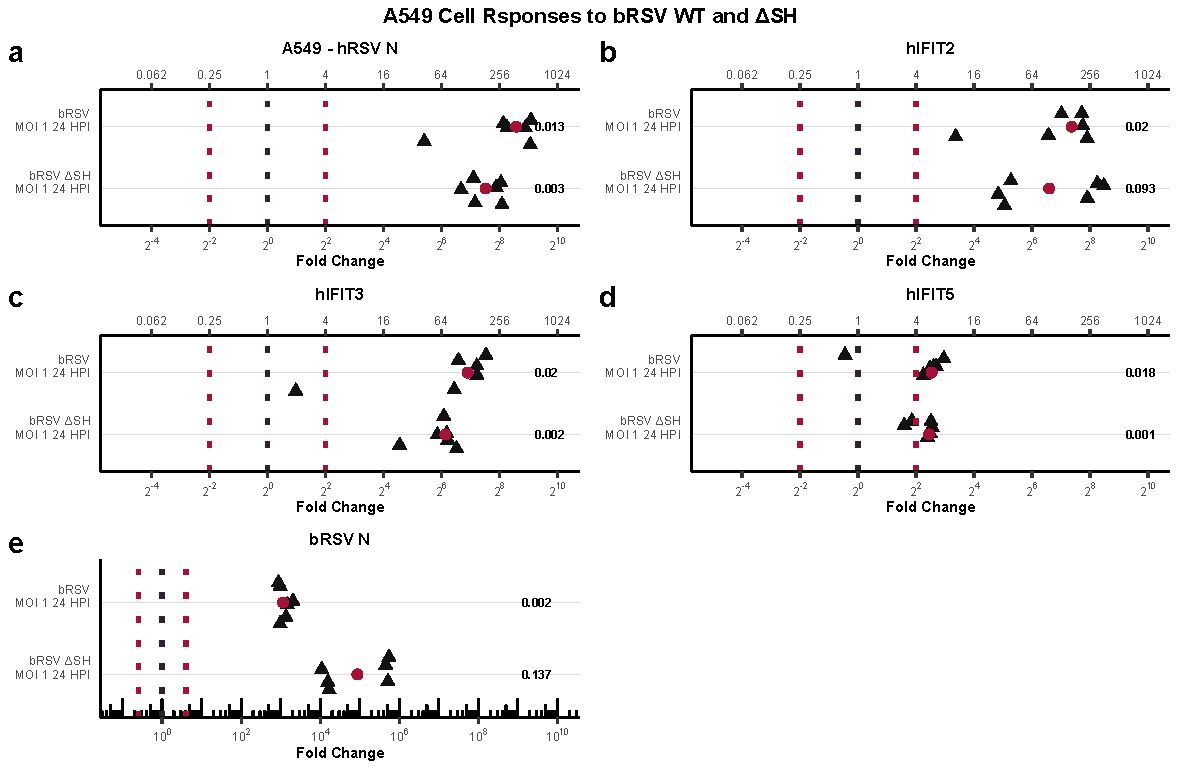
\includegraphics[width=1\linewidth]{06. Chapter 1/Figs/01. Induction/07. a549_brsv_moi1.pdf}
    \caption[A549 \textit{hIFIT} Response to WT and \(\Delta\)SH bRSV Infection.]{\textbf{A549 \textit{hIFIT} Response to WT and \(\Delta\)SH bRSV Infection.}  a) \textit{hIFIT1}, (b) \textit{hIFIT2}, (c) \textit{hIFIT3}, (d) \textit{hIFIT5}, and (e) \textit{bRSV N} gene expression levels were assessed using quantitative real-time PCR (qPCR) in A549 cell line following infection with WT or \(\Delta\)SH bRSV at MOI 1 for 24 hours post-infection. Relative expression values are normalized to standardized mock-treated samples. Median values are represented by red circles. The black dotted line represents mock expression levels, while the red dotted lines indicate biologically significant induction thresholds. Numeric values indicate the p-values compared to mock-treated samples.}
    \label{fig:Responses of A549 to bRSV WT and dSH.}
\end{figure}

The results reveal that both bovine RSV (bRSV) wild-type (WT) and bRSV \(\Delta\)SH were successful in replicating within the A549 cell line. Furthermore, these infections induced all \textit{hIFITs} to levels that are biologically significant. Interestingly, there is a noteworthy observation: despite the \(\Delta\)SH mutant virus displaying \textit{N} mRNA levels approximately two orders of magnitude higher than those of the WT bRSV, the induction magnitudes of \textit{hIFITs}, in general, were lower in the case of \(\Delta\)SH infection compared to WT bRSV infection. This finding is somewhat counterintuitive, as the absence of the SH protein should theoretically reduce the virus's infectivity, leading to weaker replication competence. Conversely, the lack of the SH protein should also result in higher \textit{ISG} induction, as there would be less antagonism of the activation cascades by the virus. Taking a closer look at the individual \textit{hIFITs}, it is evident that \textit{hIFIT1} exhibited the highest median induction levels among all \textit{hIFITs}, with values of 400-fold and 150-fold for bRSV WT and \(\Delta\)SH infections, respectively. This finding once again highlights \textit{hIFIT1} as the most strongly induced \textit{hIFIT} in response to viral infection. Conversely, \textit{hIFIT5} displayed the lowest median induction values of 6-fold for both viruses, consistent with the consistently lower induction values observed throughout the study. \textit{hIFIT2} and \textit{hIFIT3} showed median inductions of 180-fold and 80-fold for bRSV WT, and 128-fold and 70-fold for bRSV \(\Delta\)SH, respectively. Comparing these results to the previous data obtained from crude-extracted hRSV at MOI 1 and 24 HPI (Figure \ref{fig:A549 response to hRSV timepoints}), it is apparent that although the \textit{bRSV N} median relative abundances were two and one orders of magnitude lower for bRSV WT and \(\Delta\)SH, respectively, compared to \textit{hRSV N}, they induced significantly greater \textit{hIFIT} responses. This suggests that bRSV exhibits enhanced replication in human cells, likely due to the absence of species-specific inhibition mechanisms. This enhanced replication, in turn, triggers higher \textit{hIFIT} induction as a response.

\begin{figure}
    \centering
    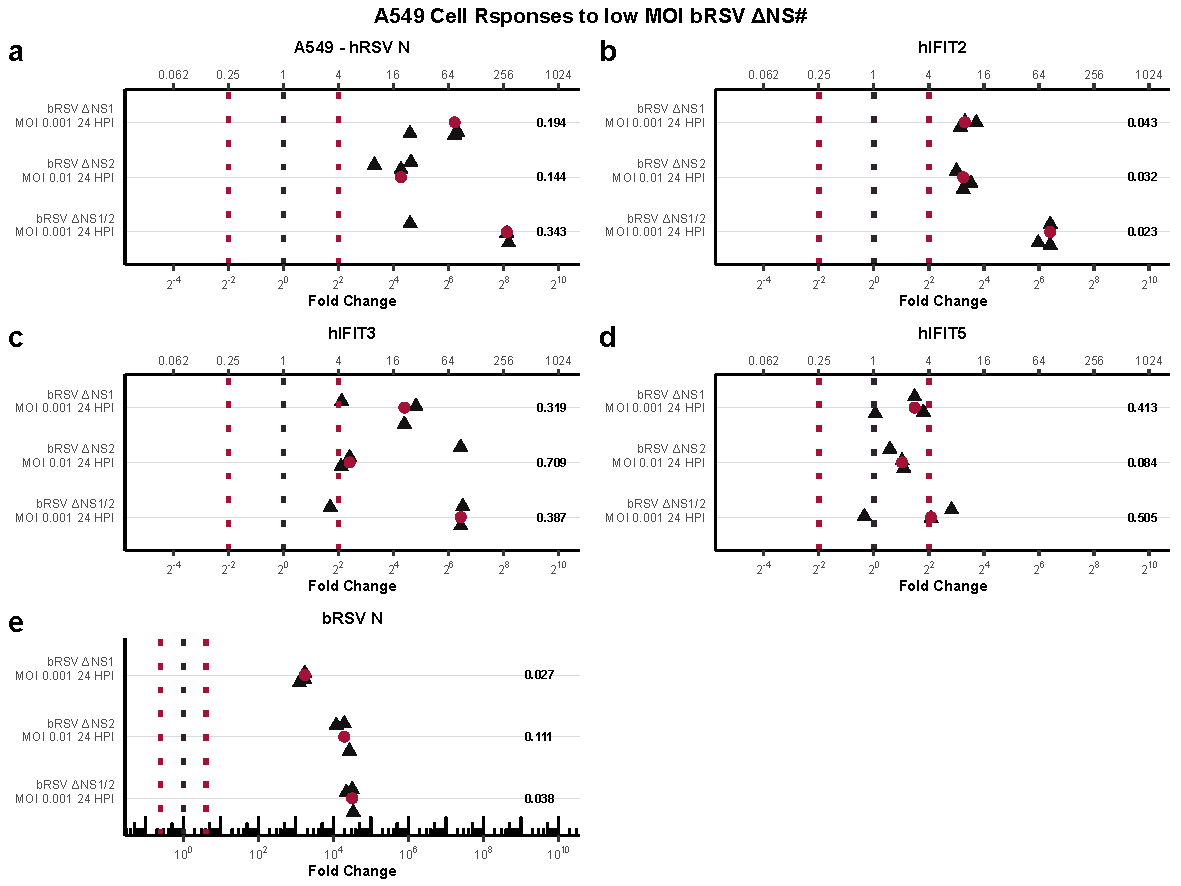
\includegraphics[width=1\linewidth]{06. Chapter 1/Figs/01. Induction/08. a549_brsv_dns.pdf}
    \caption[A549 \textit{hIFIT} Response to Low MOI \(\Delta\)NS bRSV Infections.]{\textbf{A549 \textit{hIFIT} Response to Low MOI \(\Delta\)NS bRSV Infections.} a) \textit{hIFIT1}, (b) \textit{hIFIT2}, (c) \textit{hIFIT3}, (d) \textit{hIFIT5}, and (e) \textit{bRSV N} gene expression levels were assessed using quantitative real-time PCR (qPCR) in A549 cell line following infection with bRSV \(\Delta\)NS1, \(\Delta\)NS2, and \(\Delta\)NS1/2 at MOIs of 0.001, 0.01, and 0.001 respectively. Relative expression values are normalized to standardized mock-treated samples. Median values are represented by red circles. The black dotted line represents mock expression levels, while the red dotted lines indicate biologically significant induction thresholds. Numeric values indicate the p-values compared to mock-treated samples.}
    \label{fig:Responses of A549 to bRSV dNSs.}
\end{figure}

In the subsequent phase of our investigation, we delved into the effects of other mutant bRSV viruses, specifically \(\Delta\)NS1, \(\Delta\)NS2, and a double knockout (\(\Delta\)NS1/2). As previously mentioned, we encountered challenges in achieving high viral titers using the crude-extraction method. Consequently, we employed lower multiplicities of infection (MOIs) compared to what was utilized with the WT and \(Delta\)SH bRSV strains. Specifically, we used an MOI of 0.001 for \(\Delta\)NS1 and \(\Delta\)NS1/2, and 0.01 for \(\Delta\)NS2 bRSV. Total mRNA was extracted 24 hours post-infection. In Figure \ref{fig:Responses of A549 to bRSV dNSs.}, it is evident that all three mutant viruses were capable of successful replication, despite the low MOI. The replication kinetics parallel those observed in Figure \ref{fig:Responses of A549 to bRSV WT and dSH.}, where \(\Delta\)NS1 \textit{bRSV N} mRNA levels were comparable to those in the wild-type infection, and \(\Delta\)NS2 and \(\Delta\)NS1/2 levels were akin to those seen in \(Delta\)SH bRSV infection, albeit slightly lower. Furthermore, the responses of \textit{hIFITs} were diverse but consistently displayed upregulation in all cases. \textit{hIFIT1} exhibited the highest upregulation, with a 70-fold increase in response to \(\Delta\)NS1, a 20-fold increase to \(\Delta\)NS2, and 300-fold increase to \(\Delta\)NS1/2. In contrast, \textit{hIFIT2} induction levels were nearly identical for \(\Delta\)NS1 and \(\Delta\)NS2 viruses, hovering around 8-fold, despite the difference in MOI. \(\Delta\)NS1/2 bRSV infection induced \textit{hIFIT2} the most, with a 70-fold increase. The induction dynamics of \textit{hIFIT3} revealed distinct patterns. While \(\Delta\)NS1 infection induced it to higher levels than observed for \textit{hIFIT2} (20-fold), \(\Delta\)NS2 yielded a modest induction, barely reaching biological significance at 4-fold. Strikingly, the virus lacking both non-structural proteins (\(\Delta\)NS1/2) induced \textit{hIFIT3} to levels similar to those observed with \textit{hIFIT2} (70-fold). Although we observed similar upregulation trends with \textit{hIFIT5} compared to other \textit{hIFITs}, with \(\Delta\)NS1 causing moderate induction, \(\Delta\)NS2 resulting in low induction, and \(\Delta\)NS1/2 causing high induction, only the latter can be considered biologically significant, with a 4-fold increase. Notably, in comparison to the results obtained with low MOI hRSV infection (Figure \ref{fig:A549 response to hRSV timepoints}), bRSV appeared to be more replication-competent, as indicated by the relative \textit{bRSV N} mRNA levels. Additionally, bRSV proved to be a more potent inducer of \textit{hIFITs}, whereas low MOI hRSV infection failed to elicit any detectable induction. This data also highlights the differential regulatory roles of NS1 and NS2, with NS1 exerting a more pronounced negative effect on \textit{hIFIT} induction compared to NS2. The absence of both proteins appears to exert a synergistic effect on \textit{hIFIT} induction.

\begin{figure}
    \centering
    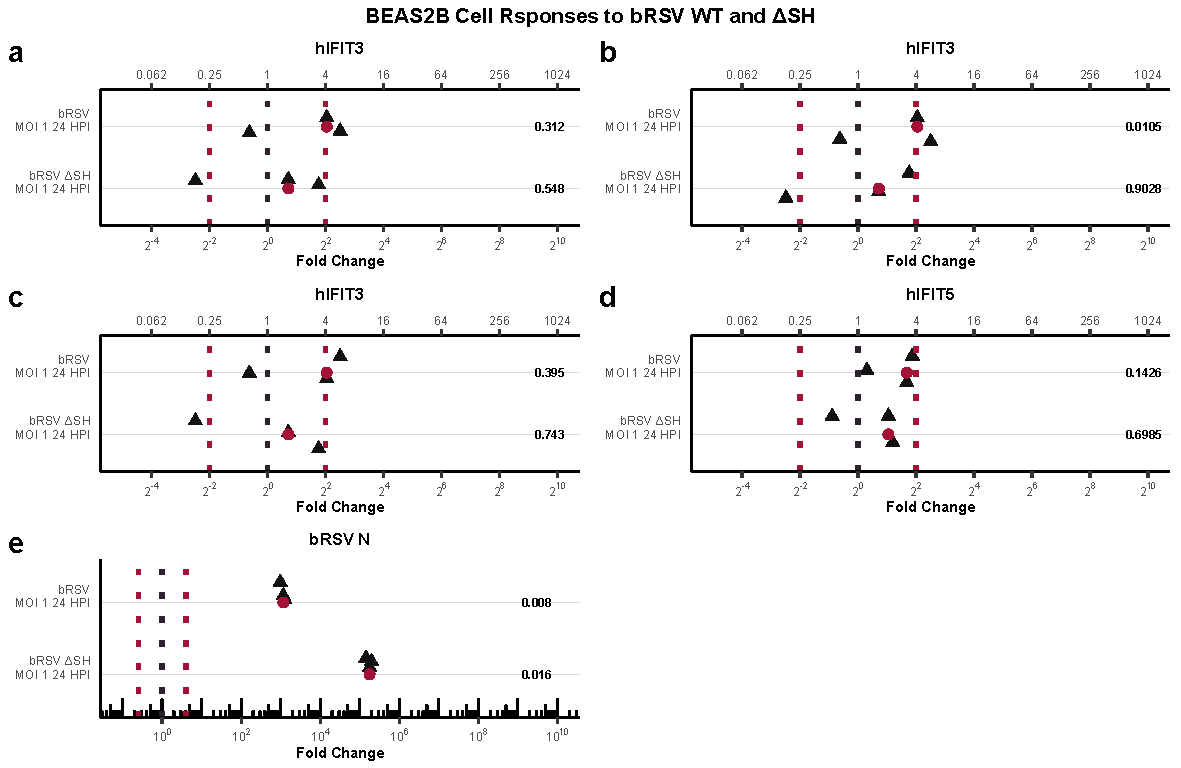
\includegraphics[width=1\linewidth]{06. Chapter 1/Figs/01. Induction/11. beas2b_brsv_moi1.pdf}
    \caption[BEAS-2B \textit{hIFIT} Response to WT and \(\Delta\)SH bRSV Infection.]{\textbf{BEAS-2B \textit{hIFIT} Response to WT and \(\Delta\)SH bRSV Infection.} a) \textit{hIFIT1}, (b) \textit{hIFIT2}, (c) \textit{hIFIT3}, (d) \textit{hIFIT5}, and (e) \textit{bRSV N} gene expression levels were assessed using quantitative real-time PCR (qPCR) in BEAS-2B cell line following infection with WT or \(\Delta\)SH bRSV at MOI 1 for 24 hours post-infection. Relative expression values are normalized to standardized mock-treated samples. Median values are represented by red circles. The black dotted line represents mock expression levels, while the red dotted lines indicate biologically significant induction thresholds. Numeric values indicate the p-values compared to mock-treated samples.}
    \label{fig:BEAS-2B responses to bRSV WT and dSH.}
\end{figure}

To validate our findings, we conducted parallel experiments in the BEAS-2B cell line, mirroring the experimental setup described earlier for A549 \textit{hIFIT} responses to bRSV infection. Figure \ref{fig:BEAS-2B responses to bRSV WT and dSH.} illustrates the induction levels resulting from infections at MOI 1, 24 hours post-infection (HPI) with both WT and \(\Delta\)SH bRSV. Based on the median relative \textit{bRSV N} mRNA levels, it is evident that these viruses can effectively infect BEAS-2B cells and replicate, achieving levels roughly equivalent to those observed in the A549 cell line. Furthermore, the main trends observed in the A549 experiments are largely recapitulated in BEAS-2B cells, with the \textit{hIFITs} displaying positive induction, with hightened sensitivity to WT bRSV infection. However, there is a notable difference in the magnitude of these inductions. Specifically, in more detail, the induction of all \textit{hIFITs} appears to be similar, but only barely reaches biological significance with WT bRSV infection (4-fold), and is notably weaker with \(\Delta\)SH infection (just over 2-fold). Intriguingly, \textit{hIFIT5} is induced just below the threshold of biological significance by WT bRSV, and at similar levels as the other \textit{hIFITs} by the mutant virus. This observation suggests an interesting phenomenon: \textit{hIFIT} induction appears to be specific to both the cell line and the stimulus, highlighting the contextual nature of this response.

\begin{figure}
    \centering
    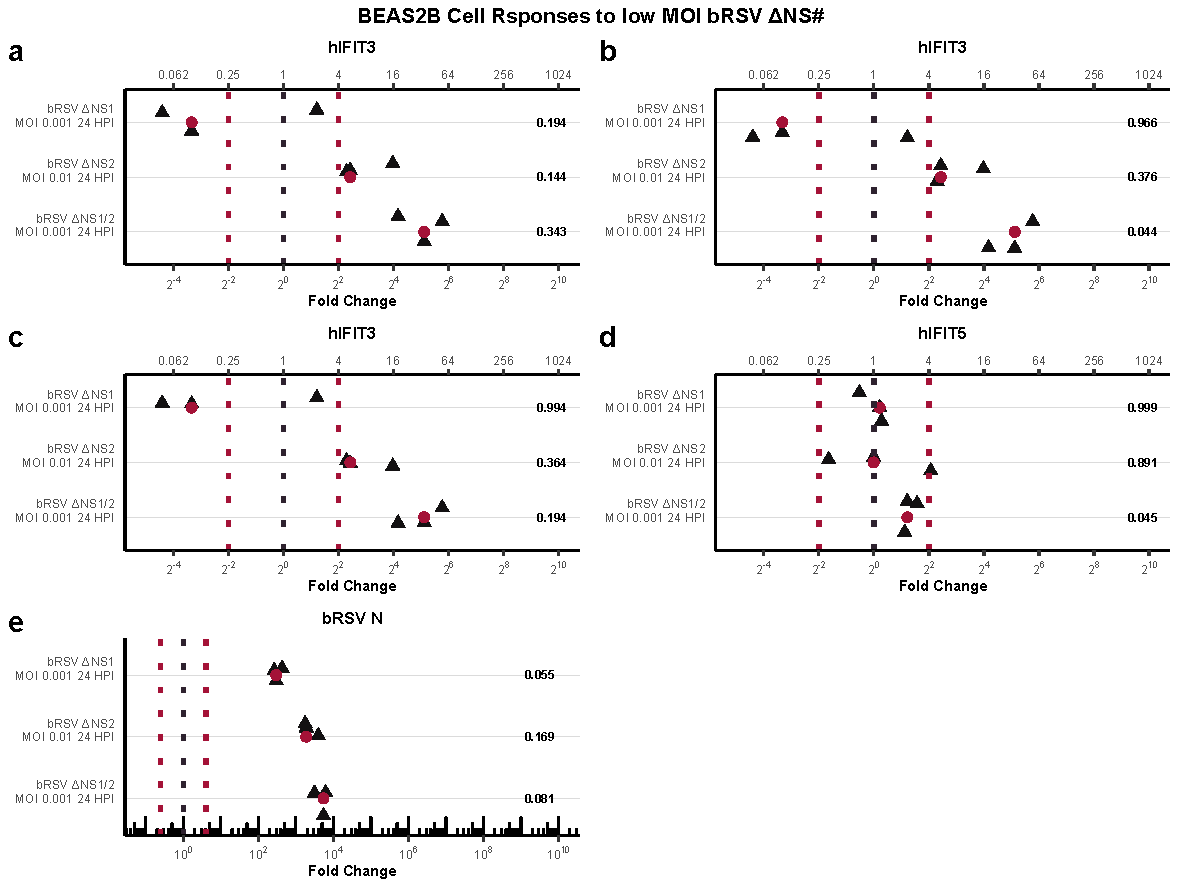
\includegraphics[width=1\linewidth]{06. Chapter 1/Figs/01. Induction/12. beas2b_brsv_dns.pdf}
    \caption[BEAS-2B \textit{hIFIT} Response to Low MOI \(\Delta\)NS bRSV Infections.]{\textbf{BEAS-2B \textit{hIFIT} Response to Low MOI \(\Delta\)NS bRSV Infections.} a) \textit{hIFIT1}, (b) \textit{hIFIT2}, (c) \textit{hIFIT3}, (d) \textit{hIFIT5}, and (e) \textit{bRSV N} gene expression levels were assessed using quantitative real-time PCR (qPCR) in BEAS-2B cell line following infection with bRSV \(\Delta\)NS1, \(\Delta\)NS2, and \(\Delta\)NS1/2 at MOIs of 0.001, 0.01, and 0.001 respectively. Relative expression values are normalized to standardized mock-treated samples. Median values are represented by red circles. The black dotted line represents mock expression levels, while the red dotted lines indicate biologically significant induction thresholds. Numeric values indicate the p-values compared to mock-treated samples.}
    \label{fig:BEAS-2B responses to bRSV dNSs.}
\end{figure}

To further validate the findings from the A549 cell line regarding \(\Delta\)NSs bRSV infections (Figure \ref{fig:Responses of A549 to bRSV dNSs.}), we conducted experiments in the BEAS-2B cell line using the same experimental protocol. Figure \ref{fig:BEAS-2B responses to bRSV dNSs.} reveals that the induction behavior in BEAS-2B cells differs from that observed in A549 cells. Based on the relative \textit{bRSV N} mRNA levels, we confirm that the mutant viruses were capable of replicating in BEAS-2B cells, although the absolute relative values are approximately one order of magnitude lower than what was observed in the A549 cell line. Interestingly, \textit{hIFIT5} does not respond to infections with \(\Delta\)NS1 and \(\Delta\)NS2 bRSV, but exhibits a positive and biologically significant response to \(\Delta\)NS1/2 virus. In contrast, \textit{hIFIT1}, \textit{hIFIT2}, and \textit{hIFIT3} display a consistent induction profile in response to these stimuli. Specifically, \(\Delta\)NS1 infection downregulates all three genes by approximately \(2^{-3}\)-fold, while \(\Delta\)NS2 infection causes a just biologically significant induction (4-fold). The double mutant \(\Delta\)NS1/2 induces a median response of 32-fold. This data suggests that the NS1 protein is inductive for \textit{hIFIT} expression, while the presence of NS2 negatively influences \textit{hIFIT} expression, in contrast to the findings in A549 cells. Moreover, the absence of both non-structural proteins seems to have a synergistically positive effect on \textit{hIFIT} induction in BEAS-2B cells, consistent with what was observed in the A549 cell line. This divergence highlights the context-dependent nature of \textit{hIFIT} induction.